%%%%%%%%%%%%%%%%%%%%%%%%%%%%%%%%%%%%%%%%%
% Beamer Presentation
% LaTeX Template
% Version 1.0 (10/11/12)
%
% This template has been downloaded from:
% http://www.LaTeXTemplates.com
%
% License:
% CC BY-NC-SA 3.0 (http://creativecommons.org/licenses/by-nc-sa/3.0/)
%
%%%%%%%%%%%%%%%%%%%%%%%%%%%%%%%%%%%%%%%%%

%----------------------------------------------------------------------------------------
%	PACKAGES AND THEMES
%----------------------------------------------------------------------------------------

\documentclass{beamer}

\mode<presentation> {

% The Beamer class comes with a number of default slide themes
% which change the colors and layouts of slides. Below this is a list
% of all the themes, uncomment each in turn to see what they look like.

%\usetheme{default}
%\usetheme{AnnArbor}
%\usetheme{Antibes}
%\usetheme{Bergen}
%\usetheme{Berkeley}
%\usetheme{Berlin}
%\usetheme{Boadilla}
%\usetheme{CambridgeUS}
%\usetheme{Copenhagen}
%\usetheme{Darmstadt}
%\usetheme{Dresden}
%\usetheme{Frankfurt}
%\usetheme{Goettingen}
%\usetheme{Hannover}
%\usetheme{Ilmenau}
%\usetheme{JuanLesPins}
%\usetheme{Luebeck}
\usetheme{Madrid}
%\usetheme{Malmoe}
%\usetheme{Marburg}
%\usetheme{Montpellier}
%\usetheme{PaloAlto}
%\usetheme{Pittsburgh}
%\usetheme{Rochester}
%\usetheme{Singapore}
%\usetheme{Szeged}
%\usetheme{Warsaw}

% As well as themes, the Beamer class has a number of color themes
% for any slide theme. Uncomment each of these in turn to see how it
% changes the colors of your current slide theme.

%\usecolortheme{albatross}
%\usecolortheme{beaver}
%\usecolortheme{beetle}
%\usecolortheme{crane}
%\usecolortheme{dolphin}
%\usecolortheme{dove}
%\usecolortheme{fly}
%\usecolortheme{lily}
%\usecolortheme{orchid}
%\usecolortheme{rose}
%\usecolortheme{seagull}
%\usecolortheme{seahorse}
%\usecolortheme{whale}
%\usecolortheme{wolverine}

%\setbeamertemplate{footline} % To remove the footer line in all slides uncomment this line
%\setbeamertemplate{footline}[page number] % To replace the footer line in all slides with a simple slide count uncomment this line

%\setbeamertemplate{navigation symbols}{} % To remove the navigation symbols from the bottom of all slides uncomment this line
}

\usepackage{graphicx} % Allows including images
\usepackage{booktabs} % Allows the use of \toprule, \midrule and \bottomrule in tables
\usepackage[utf8]{inputenc}
\usepackage[brazilian]{babel}

\setlength{\parskip}{1em}

\newtheorem{teo}{Teorema}
\newtheorem{lema}{Lema}

\theoremstyle{definition}
\newtheorem{exe}{Exemplo}
\newtheorem{defi}{Definição}
\newtheorem{obs}{Observação}
\newtheorem{prop}{Proposição}

%----------------------------------------------------------------------------------------
%	TITLE PAGE
%----------------------------------------------------------------------------------------

\title[Sistemas fuzzy e métodos de ativação]{Estudos teóricos e práticos sobre sistemas fuzzy baseados em regras e 
métodos de ativação} % The short title appears at the bottom of every slide, the full title is only on the title page

\author[Renato Lopes Moura]{Renato Lopes Moura \\[5ex] 
\small Orientador: Peter Sussner} % Your name
\institute[Unicamp] % Your institution as it will appear on the bottom of every slide, may be shorthand to save space
{
Universidade Estadual de Campinas \\ % Your institution for the title page
\medskip
\textit{ra163050@ime.unicamp.br} % Your email address
}
\date{\today} % Date, can be changed to a custom date

\begin{document}
\AtBeginSection[]
  {
     \begin{frame}<beamer>
     \frametitle{Organização do trabalho}
     \tableofcontents[currentsection]
     \end{frame}
  }

\setlength{\abovedisplayskip}{10pt}
\setlength{\belowdisplayskip}{10pt}

\begin{frame}
\titlepage % Print the title page as the first slide
\end{frame}

\begin{frame}
\frametitle{Organização do trabalho} % Table of contents slide, comment this block out to remove it
\tableofcontents % Throughout your presentation, if you choose to use \section{} and \subsection{} commands, these will automatically be printed on this slide as an overview of your presentation
\end{frame}

%----------------------------------------------------------------------------------------
%	PRESENTATION SLIDES
%----------------------------------------------------------------------------------------
\section{Introdução}

\begin{frame}
\frametitle{Introdução}
%This work presents the Moser-Navara axioms, that is an attempt of axiomatization of the design of Fuzzy Inference Systems (FIS) that has a mathematical foundation instead of just basing in empirical results. Different FIS designs using conjunctive and implicative models and their link with Mathematical Morphology theory will be explored as well as their adherence to the aforementioned axioms. Finally, there are some experimental results of different FIS designs and a comparison of their performances.
Este trabalho pretende fazer um estudo sobre sistemas de inferência \textit{fuzzy} observando os modelos conjuntivo e implicativo de equações relacionais \textit{fuzzy} e diferentes regras de composição de relações \textit{fuzzy}.\par
Também serão estudados diferentes métodos de ativação de regras nos sistemas de inferência, baseado nos trabalhos de Peter Sussner e Estevão Laureano em Memórias Associativas Morfológicas. Mais especificamente S-FAMs e E-FAMs, que utilizam medidas de subsethood e equivalência respectivamente.\par
Os axiomas de Moser-Navara fornecem uma fundamentação matemática para avaliar a coerência de um sistema de inferência. Posteriormente este trabalho foi expandido por Martin Stepnicka \textit{et al}. para avaliar outros modelos de inferência além do tradicional proposto por Mamdani-Assilian. Aqui, faremos uma revisão teórica destes resultados e analisaremos o comportamento dos sistemas de inferência em problemas práticos de classificação e regressão.
\end{frame}

%------------------------------------------------

\section{Conceitos matemáticos}

%Acho que deveria vir um slide antes disso falando sobre como a lógica fuzzy é uma extensão da lógica clássica
\begin{frame}
\frametitle{Operações fuzzy}
Estendendo os operadores lógicos booleanos para o domínio \textit{fuzzy} podemos obter uma família de operações entre conjuntos \textit{fuzzy} que modelam as operações de conjunção (AND) e disjunção (OR)\cite{p6}\cite{p5}.\par
Uma conjunção \textit{fuzzy} é uma função $C:[0,1] \times [0,1] \rightarrow [0,1]$ tal que $C(0,0) = C(1,0) = C(0,1) = 0$ e $C(1,1) = 1$.\par
Se além disso, esta função for \underline{comutativa}, \underline{associativa} e satisfizer $C(1,a) = a$ para todo $a \in [0,1]$, então $C$ é chamada \underline{t-norma}.\par
Da mesma forma, pode ser definida uma disjunção \textit{fuzzy} como uma função $D:[0,1] \times [0,1] \rightarrow [0,1]$ tal que $D(0,0) = 0$ e $D(1,0) = D(0,1) = D(1,1) = 1$. Similarmente, se $D$ for uma função \underline{comutativa}, \underline{associativa} e satisfizer $D(0,a) = a$ para todo $a \in [0,1]$, então $D$ é chamada \underline{t-conorma} ou \underline{s-norma}.\par
\end{frame}

\begin{frame}
\frametitle{Operações fuzzy}
Outro operador que pode ser estendido da lógica booleana é o operador de implicação. Uma implicação \textit{fuzzy} é uma função $I:[0,1] \times [0,1] \rightarrow [0,1]$ onde $I(0,0) = I(0,1) = I(1,1) = 1$ e $I(1,0) = 0$.\par
Um tipo especial de implicação pode ser construído utilizando-se t-normas que sejam contínuas à esquerda, ou seja:
\begin{align*}
\lim_{n\to\infty} T(x_{n},y) = T(\lim_{n\to\infty} x_{n},y) 
\end{align*}
Então é possível definir a implicação associada à t-norma T como:
\begin{align*}
I_{T}(a,b) = \bigvee \{c \in [0,1]|T(a,c) \leq b\}
\end{align*}
Esta implicação $I_{T}$ é chamada \underline{implicação residual \textit{fuzzy}} (ou R-implicação).
\end{frame}

\begin{frame}
\frametitle{Relações fuzzy}
Uma relação binária pode ser vista como a associação (ou a ausência dela) entre elementos de dois conjuntos. Uma relação binária \textit{fuzzy} é uma extensão deste conceito para conjuntos \textit{fuzzy}.\par
Formalmente, segundo \cite{p3} temos:
\begin{defi}
Uma relação binária \textit{fuzzy} sobre $\mathcal{F}(X)$ é uma relação $\mathcal{R}$ sobre $\mathcal{F}(X)\times\mathcal{F}(X)$ definida por uma função de pertinência:
\begin{center}
$\mathcal{R}:\mathcal{F}(X)\times\mathcal{F}(X) \rightarrow [0,1]$
\end{center}
\end{defi}
\end{frame}

\begin{frame}
\frametitle{Medida de Subsethood}
Um exemplo importante de relação binária \textit{fuzzy} é a medida de \textit{subsethood}. Uma medida de \textit{subsethood} avalia o grau de "inclusão" de um conjunto \textit{fuzzy} em outro, em outras palavras é uma generalização do operador $\subseteq$ da teoria de conjuntos clássica.\par
Neste trabalho adotaremos a seguinte definição de medida de \textit{subsethood} proposta por \cite{p7}:
\begin{defi}
 Seja uma função $S:\mathcal{F}(X)\times\mathcal{F}(X) \rightarrow [0,1]$. $S(A,B)$ é uma medida de \textit{subsethood} se para $A,B,C \in \mathcal{F}(X)$ temos:
 \begin{enumerate}
 \item $S(A,B)=1 \Leftrightarrow A \subseteq B$ 
 \item $S(X,\emptyset)=0$ 
 \item Se $A \subseteq B \subseteq C$, então $S(C,A) \leq S(B,A)$ e $S(C,A) \leq S(C,B)$
\end{enumerate}
\end{defi}
\end{frame}

\begin{frame}
\frametitle{Medida de Similaridade}
Outra importante relação entre conjuntos \textit{fuzzy} é a medida de similaridade, que generaliza a igualdade de conjuntos da teoria de conjuntos clássica.
Neste trabalho utilizaremos a definição mais comum de medida de similaridade encontrada na literatura (que também pode ser encontrada como a definição de uma medida de equivalência).
\begin{defi}
Uma função $SM:\mathcal{F}(X)\times\mathcal{F}(X) \rightarrow [0,1]$ é dita uma medida de similaridade se $SM$ satisfaz as seguintes propriedades para todos $A, B, C \in \mathcal{F}(X)$:
\begin{enumerate}
\item $SM(A,B) = SM(B,A)$
\item $SM(X,\emptyset) = 0$
\item $SM(A,A) = 1$
\item Se $A \subseteq B \subseteq C$, então $SM(A,B) \geq SM(A,C)$ e $SM(B,C) \geq SM(A,C)$
\end{enumerate}
\end{defi}
\end{frame}

\begin{frame}
\frametitle{Modelos de relações fuzzy}
\begin{block}{Modelo conjuntivo}
\begin{center}
$R^{\vee}_{\ast}(x,y) = \bigvee (A_{i}(x) \ast B_{i}(y))$
\end{center}
onde $\ast$ é uma t-norma contínua à esquerda.
\end{block}

\begin{block}{Modelo implicativo}
\begin{center}
$R^{\wedge}_{\rightarrow}(x,y) = \bigwedge (A_{i}(x) \rightarrow B_{i}(y))$
\end{center}
onde $\rightarrow$ é uma implicação residual.
\end{block}
\end{frame}

%------------------------------------------------

\begin{frame}
\frametitle{Composições fuzzy}
\end{frame}

\begin{frame}
\frametitle{Composições fuzzy}
\begin{block}{Regra de Composição de Inferência (composição sup-$\ast$) \cite{p15}}
\begin{center}
$B'(y) = (A' \circ R)(y) = \bigvee (A'(x) \ast R(x,y))$
\end{center}
\end{block}

\begin{block}{Subproduto de Bandler-Kohout (composição inf-$\rightarrow$) [W.Bandler, L.J.Kohout, ~70s]}
\begin{center}
$B'(y) = (A' \vartriangleleft R)(y) = \bigwedge (A'(x) \rightarrow R(x,y))$
\end{center}
\end{block}
\end{frame}

\begin{frame}
\frametitle{Composições fuzzy}
\end{frame}

%------------------------------------------------

\begin{frame}
\frametitle{Composição inf-$\rightarrow$ (Subproduto de Bandler-Kohout)}
A composição inf-$\rightarrow$ foi sugerida como um método de inferência por W. Pedrycz em \cite{p17}.\par
Entretanto, devido à popularidade alcançada pelo modelo de Mamdani-Assilian em aplicações práticas, ela acabou sendo pouco estudada.\par
Mais recentemente, esta composição teve suas propriedades estudadas em \cite{p2} e se mostrou tão adequada quanto a Regra de Composição de Inferência de Zadeh, desde que corretamente combinada com o modelo de relações \textit{fuzzy} utilizado.
\end{frame}

%------------------------------------------------

\section{Sistemas fuzzy baseados em regras}

\begin{frame}
\frametitle{Modus Ponens}
Na lógica proposicional, o \textit{modus ponens} é uma forma de raciocínio que utiliza como base uma regra de inferência para gerar conclusões a partir de fatos. Ele pode ser representado da seguinte forma:
\begin{table}[H]
\centering
\label{modus-ponens}
\begin{tabular}{ll}
\textbf{Regra:}      & "Se x é A, então y é B" \\
\textbf{Fato:}      & "x é A"                 \\
\textbf{Conclusão:} & "y é B"                
\end{tabular}
\end{table}
\end{frame}

\begin{frame}
\frametitle{Modus Ponens Generalizado}
Em contrapartida, o \textit{modus ponens generalizado} utiliza as ferramentas da teoria de conjuntos \textit{fuzzy} para aumentar o poder de inferência do \textit{modus ponens} tradicional dando origem ao chamado raciocínio aproximado. Ele pode ser representado da seguinte forma:
\begin{table}[H]
\centering
\label{modus-ponens-generalizado}
\begin{tabular}{ll}
\textbf{Regra:}      & "Se x é A, então y é B" \\
\textbf{Fato:}      & "x é A' "                 \\
\textbf{Conclusão:} & "y é B' "                
\end{tabular}
\end{table}
\end{frame}

\begin{frame}
\frametitle{Interpretação da base de regras}
Considerando o \textit{modus ponens generalizado} onde cada regra é vista como uma relação entre conjuntos fuzzy, cabem duas interpretações para uma base de regras: uma para o modelo conjuntivo e uma para o modelo implicativo de relações \textit{fuzzy}.\par
Relembrando o modelo conjuntivo de relações \textit{fuzzy} é dado por:
\begin{center}
$R^{\vee}_{\ast}(x,y) = \bigvee (A_{i}(x) \ast B_{i}(y))$
\end{center}
Desta forma a base de regras pode ser interpretada como:
\begin{table}[H]
\centering
\label{base-de-regras-conjuntivo}
\begin{tabular}{ll}
\textbf{$R1$:}      & "$x$ é $A_{1}$ \textbf{e} $y$ é $B_{1}$" \\
      & \textbf{ou}                 \\
      & ...                 \\
      & \textbf{ou}                 \\     
\textbf{$Rn$:} & "$x$ é $A_{1}$ \textbf{e} $y$ é $B_{n}$"                
\end{tabular}
\end{table}
\end{frame}

\begin{frame}
\frametitle{Interpretação da base de regras}
Citando \cite{p4}:
\begin{quote}
It seems that fuzzy rules modeled this way are not viewed as constraints, but are considered to be pieces of data. Then, the maximum expresses accumulation of data.
\end{quote}
Que em tradução livre quer dizer:
\begin{quote}
Parece que as regras fuzzy modeladas desta maneira não são vistas como restrições, mas sim como pedaços de informação. Então, a agregação pelo máximo expressa acumulação de informação.
\end{quote}
\end{frame}

\begin{frame}
\frametitle{Interpretação da base de regras}
Por outro lado, o modelo implicativo de relações \textit{fuzzy} é dado por:
\begin{center}
$R^{\wedge}_{\rightarrow}(x,y) = \bigwedge (A_{i}(x) \rightarrow B_{i}(y))$
\end{center}
Desta forma a base de regras pode ser interpretada como:
\begin{table}[H]
\centering
\label{base-de-regras-implicativo}
\begin{tabular}{ll}
\textbf{$R1$:}      & "Se $x$ é $A_{1}$ \textbf{então} $y$ é $B_{1}$" \\
      & \textbf{e}                 \\
      & ...                 \\
      & \textbf{e}                 \\     
\textbf{$Rn$:} & "Se $x$ é $A_{1}$ \textbf{então} $y$ é $B_{n}$"                
\end{tabular}
\end{table}
\end{frame}

\begin{frame}
\frametitle{Interpretação da base de regras}
Novamente citando \cite{p4}:
\begin{quote}
In the above view, each piece of information (fuzzy rule) is viewed as a constraint. This view naturally leads to a conjunctive way of merging the individual pieces of information since the more information, the more constraints and the less possible values to satisfy them.
\end{quote}
Que em tradução livre quer dizer:
\begin{quote}
Nesta visão, cada pedaço de informação (regra fuzzy) é vista como uma restrição. Esta visão naturalmente leva a uma maneira conjuntiva de agregação dos pedaços individuais de informação uma vez que quanto mais informação, mais restrições e menos valores possíveis que as satisfazem.
\end{quote}
\end{frame}
%------------------------------------------------

\section{Métodos de ativação de regras fuzzy}

\begin{frame}
\frametitle{Métodos de ativação de regras fuzzy}
Recentemente, surgiram alguns trabalhos sugerindo métodos de ativação de regras \textit{fuzzy} baseados em medidas de Subsethood e Similaridade \cite{p10} \cite{p11} \cite{p8} \cite{p9}.\par
A discussão de tais métodos faz mais sentido no contexto em que as entradas do sistema de inferência são conjuntos \textit{fuzzy}. Neste trabalho, o foco será no estudo deste caso em particular, deixando o caso de entradas \textit{crisp} não fuzzificadas para trabalhos futuros.\par
\end{frame}

\begin{frame}
\frametitle{Métodos de ativação de regras fuzzy}
Além disso, o caso \textit{crisp} independe do modelo de inferência adotado pois para um dado $x' \in X$ e $A'$ um singleton em $x'$ temos:
\begin{center}
$(A' \circ R)(y) = (A' \vartriangleleft R)(y) = R(x',y), y \in Y$
\end{center}
\end{frame}

\begin{frame}
\frametitle{Método de ativação tradicional}
Relembrando o esquema clássico de um sistema de inferência \textit{fuzzy}:
\begin{figure}[H]
 \centering
  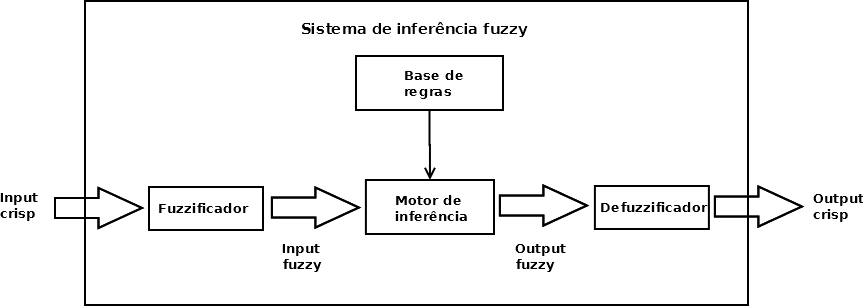
\includegraphics[width=0.8\textwidth]{FIS.png}
  \caption{Sistema de inferência \textit{fuzzy}.}
  \label{fig:FIS}
\end{figure}
\end{frame}

\begin{frame}
\frametitle{Método de ativação tradicional}
Dada uma entrada \textit{crisp} $x' \in X$ no sistema de inferência, temos a seguinte sequência de passos:
\begin{enumerate}
\item A entrada $x'$ é fuzzificada para um conjunto \textit{fuzzy} $A'(x) \in \mathcal{F}(X)$ com $A'(x')=1$
\item Para cada regra $R_{i}$ com antecedente $A_{i}$ é calculado $\alpha_{i} = \bigvee\limits_{x \in X} [A'(x) \wedge A_{i}(x)]$
\item O valor de $\alpha_{i}$ representa o grau de ativação da regra $R_{i}$
\end{enumerate}
\underline{Obs:} para simplificar a notação, os passos descritos acima descrevem um cenário onde as regras possuem um antecedente e um consequente apenas. 
\end{frame}

\begin{frame}
\frametitle{Casos onde a ativação por similaridade é superior}
Como é possível observar na figura a seguir, temos um caso onde entradas claramente diferentes produzem o mesmo grau de ativação de uma determinada regra no sistema de inferência \textit{fuzzy} de Mamdani-Assilian.\par
\begin{figure}[H]
 \centering
  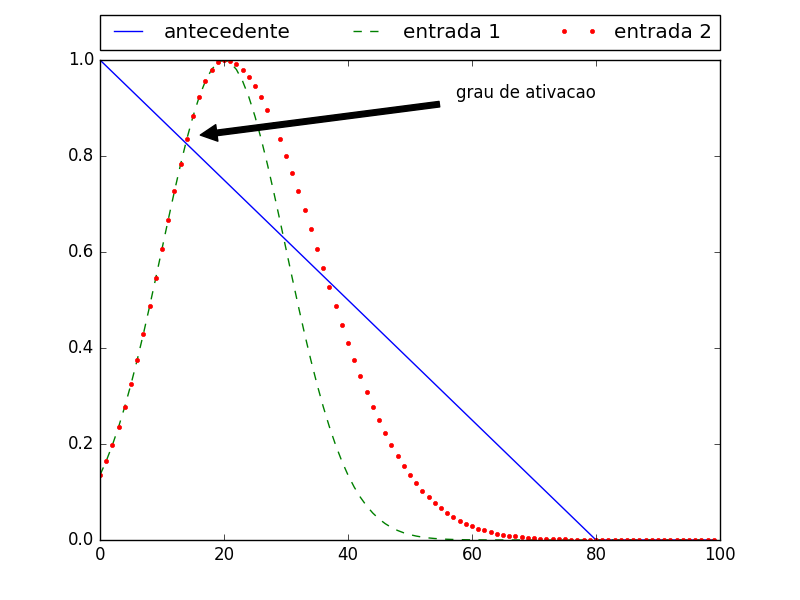
\includegraphics[width=0.5\textwidth]{ativacao_mamdani.png}
  \caption{Problema de ativação de regras no sistema de Mamdani-Assilian.}
  \label{fig:problema_mamdani}
\end{figure}
\end{frame}

\begin{frame}
\frametitle{Ativação de regras fuzzy utilizando medidas de similaridade}
Este problema foi a principal motivação para a busca por outras abordagens, como a ativação por centróide \cite{p12} \cite{p13} e por similaridade \cite{p8}.\par
Desta forma, a abordagem de ativação por uma medida de similaridade $SM(A,B) \in \mathcal{F}(X)\times\mathcal{F}(X)$ pode ser expressa matematicamente por:
\begin{center}
$B'(y) = \bigvee (SM(A'(x),A_{i}(x)) \wedge B_{i}(y))$
\end{center}
\begin{center}
ou
\end{center}
\begin{center}
$B'(y) = \bigwedge (SM(A'(x),A_{i}(x)) \rightarrow B_{i}(y))$
\end{center}
dependendo da composição de inferência escolhida.
\end{frame}

\begin{frame}
\frametitle{Casos onde a ativação por subsethood é superior}
A ativação de regras por medida de similaridade apesar de ser intuitivamente melhor do que o modelo mais comumente utilizado, ainda apresenta seus problemas, como é o caso exposto na figura a seguir.
\begin{figure}[H]
 \centering
  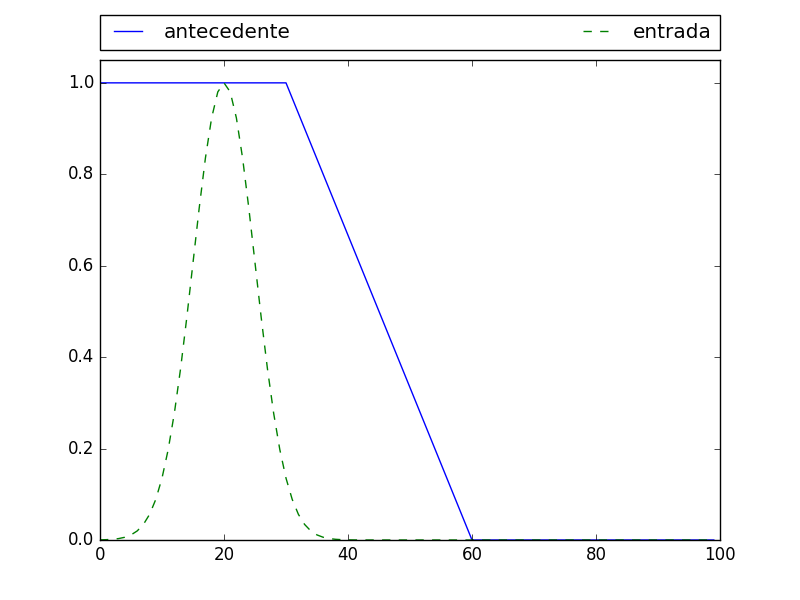
\includegraphics[width=0.5\textwidth]{problema_similaridade.png}
  \caption{Problema de ativação de regras por similaridade.}
  \label{fig:problema_similaridade}
\end{figure}
\end{frame}

\begin{frame}
\frametitle{Ativação de regras fuzzy utilizando medidas de subsethood}
Similar à abordagem de ativação por uma medida de similaridade, a ativação por uma medida de subsethood $S(A,B) \in \mathcal{F}(X)\times\mathcal{F}(X)$ pode ser expressa matematicamente por:
\begin{center}
$B'(y) = \bigvee (S(A'(x),A_{i}(x)) \wedge B_{i}(y))$
\end{center}
\begin{center}
ou
\end{center}
\begin{center}
$B'(y) = \bigwedge (S(A'(x),A_{i}(x)) \rightarrow B_{i}(y))$
\end{center}
dependendo da composição de inferência escolhida.
\end{frame}

%------------------------------------------------

\section{Axiomas de Moser-Navara} % Sections can be created in order to organize your presentation into discrete blocks, all sections and subsections are automatically printed in the table of contents as an overview of the talk
%------------------------------------------------
%\subsection{Subsection Example} % A subsection can be created just before a set of slides with a common theme to further break down your presentation into chunks

\begin{frame}
\frametitle{Axiomas de Moser-Navara}
Como ressaltado em \cite{p2}, a escolha dos objetos envolvidos (modelo de relação \textit{fuzzy}, conjuntos \textit{fuzzy}, inferência, operações matemáticas) não deve ser arbitrária. Tendo em vista os resultados empíricos obtidos ao longo dos anos, deve haver uma axiomatização natural para esta combinação.\par
Tal axiomatização foi proposta em \cite{p14}.
\end{frame}

\begin{frame}
\frametitle{Axiomas de Moser-Navara}
\begin{enumerate}
\item Para todo $i \in {1,\dots,n}$
\begin{center}
$A_{i} \circ R^{\vee}_{\ast} = B_{i}$
\end{center}

\hfill

\item Para cada \textit{input} normal $A' \in \mathcal{F}(X)$ existe um índice $i$ tal que
\begin{center}
$A' \circ R^{\vee}_{\ast} \nsubseteq B_{i}$
\end{center}

\hfill

\item O \textit{output} $A' \circ R^{\vee}_{\ast}$ pertence à união dos consequentes $B_{i}$ de regras ativadas
\begin{center}
$A' \circ R^{\vee}_{\ast} \subseteq \bigcup\limits_{i \in F} B_{i}$\\
$F = \{i|Supp(A_{i})\cap Supp(A') \neq \emptyset\}, (B_{i} \cup B_{j})(y) = B_{i}(y) \vee B_{j}(y)$
\end{center}
\end{enumerate}
\end{frame}

%------------------------------------------------

\begin{frame}
\frametitle{Interpretação dos axiomas}
Uma interpretação literal destes axiomas dada em \cite{p2} é a seguinte:
\begin{enumerate}
\item A relação fuzzy $R(x,y)$ deve apresentar \textit{recall} (preservação do \textit{modus ponens} ou interpolação \textit{fuzzy})

\hfill

\item Para \textit{inputs} normais, o sistema deve apresentar \textit{outputs} significativos com informação não-trivial

\hfill

\item Se o \textit{input} do sistema está contido no universo dos antecedentes, então deve existir um \textit{output} não-nulo para ele
\end{enumerate}
\end{frame}

%------------------------------------------------

\begin{frame}
\frametitle{Axiomas de Moser-Navara}
Com base nesta interpretação, foram propostos axiomas similares para o caso da composição inf-$\rightarrow$ \cite{p2}
\begin{enumerate}
\item Para todo $i \in {1,\dots,n}$
\begin{center}
$A_{i} \vartriangleleft R^{\wedge}_{\rightarrow} = B_{i}$
\end{center}

\hfill

\item Para cada \textit{input} normal $A' \in \mathcal{F}(X)$ existe um índice $i$ tal que
\begin{center}
$A' \vartriangleleft R^{\wedge}_{\rightarrow} \nsupseteq B_{i}$
\end{center}

\hfill

\item O \textit{output} $A' \vartriangleleft R^{\wedge}_{\rightarrow}$ contêm a interseção dos consequentes $B_{i}$ de regras ativadas
\begin{center}
$A' \vartriangleleft R^{\wedge}_{\rightarrow} \supseteq \bigcap\limits_{i \in F} B_{i}$\\
$F = \{i|Supp(A_{i})\cap Supp(A') \neq \emptyset\}, (B_{i} \cap B_{j})(y) = B_{i}(y) \wedge B_{j}(y)$
\end{center}
\end{enumerate}
\end{frame}

%------------------------------------------------

\begin{frame}
\frametitle{Combinação de $R^{\vee}$ e $\circ$}
Relembrando um resultado de \cite{p18}, temos o seguinte teorema:
\begin{block}{Teorema}
Sejam $A_{i}$, para $i=1,...,n$ conjuntos \textit{fuzzy} normais. Então $R^{\vee}$ é uma solução de
\begin{center}
$A_{i} \circ R = B_{i}, i=1,...,n$
\end{center}
se, e somente se, a seguinte condição é válida para $i,j \in \{1,...,n\}$ arbitrários
\begin{center}
$\bigvee\limits_{x \in X} (A_{i}(x) \ast A_{j}(x)) \leq \bigwedge\limits_{y \in Y} (B_{i}(y) \leftrightarrow B_{j}(y))$
\end{center}
\end{block}
\end{frame}

%------------------------------------------------

\begin{frame}
\frametitle{Combinação de $R^{\vee}$ e $\circ$}
\begin{block}{Proposição \cite{p14}}
Seja $\ast$ uma t-norma sem divisores de zero. Seja todos $A_{i}, i=1,...,n$ contínuos e normais e sejam $B_{i}, i=1,...,n$ conjuntos \textit{fuzzy} com \textbf{suportes mutuamente diferentes}. Então a combinação de $R^{\vee}$ e $\circ$ não satisfaz os axiomas 1 e 2 simultaneamente.
\end{block}
Suportes mutuamente diferentes de $B_{i} \Rightarrow \bigwedge\limits_{y \in Y} (B_{i}(y) \leftrightarrow B_{j}(y)) = 0$\par
$\bigvee\limits_{x \in X} (A_{i}(x) \ast A_{j}(x))$ deve ser igual a 0 $\Rightarrow$ $A_{i}$ devem ser disjuntos!
\end{frame}

%------------------------------------------------

\begin{frame}
\frametitle{Combinação de $R^{\wedge}$ e $\vartriangleleft$}
Um resultado semelhante para a combinação de $R^{\wedge}$ e $\vartriangleleft$ foi proposto em \cite{p16}.
\begin{block}{Proposição \cite{p16}}
Seja $\ast$ uma t-norma sem divisores de zero. Seja todos $A_{i}, i=1,...,n$ contínuos e normais e sejam $B_{i}, i=1,...,n$ conjuntos \textit{fuzzy} com \textbf{suportes mutuamente diferentes}. Então a combinação de $R^{\wedge}$ e $\vartriangleleft$ não satisfaz os axiomas 1 e 2 simultaneamente.
\end{block}
A demonstração segue a mesma linha uma vez que a idéia original dos axiomas não foi modificada para o caso da composição inf-$\rightarrow$.
\end{frame}

%------------------------------------------------

\begin{frame}
\frametitle{Consequências}
Diante dos problemas apresentados, as combinações mais seguras de modelos de relações \textit{fuzzy} e métodos de inferência são:
\begin{itemize}
\item $R^{\wedge}$ (modelo implicativo) e $\circ$ (composição sup-t)
\item $R^{\vee}$ (modelo conjuntivo) e $\vartriangleleft$ (composição inf-$\rightarrow$)
\end{itemize}
Apesar disso, essas combinações são pouco utilizadas.
\end{frame}

%------------------------------------------------

\section{Estudos de caso}

%\begin{frame}
%\frametitle{Regras esparsas}
%\end{frame}

\begin{frame}
\frametitle{Previsão de séries temporais}
\end{frame}

\begin{frame}
\frametitle{Sensor de estacionamento}
\end{frame}

%------------------------------------------------
\section{Conclusão}

\begin{frame}
\frametitle{Conclusão}
\end{frame}

%------------------------------------------------
%\section{Trabalhos futuros}

%\begin{frame}
%\frametitle{Trabalhos futuros}
%\end{frame}

%------------------------------------------------
%------------------------------------------------
%------------------------------------------------

\begin{frame}
\frametitle{Referências}
\footnotesize{
\begin{thebibliography}{99} % Beamer does not support BibTeX so references must be inserted manually as below
\bibitem[Stepnicka \textit{et al.}, 2010]{p1} Martin Stepnicka, Bernard de Baets and Lenka Noskova (2010)
\newblock Arithmetic Fuzzy Models
\newblock \emph{IEEE Transactions on Fuzzy Systems} Vol. 18, No. 6

\bibitem[Stepnicka e Jayaram, 2010]{p2} Martin Stepnicka and Balasubramaniam Jayaram (2010)
\newblock On the Suitability of the Bandler-Kohout Subproduct as an Inference Mechanism
\newblock \emph{IEEE Transactions on Fuzzy Systems} Vol. 18, No. 2

\bibitem[Barros e Bassanezi, 2010]{p3} L.C.Barros and R.C.Bassanezi (2010)
\newblock Tópicos de Lógica Fuzzy e Biomatemática
\newblock \emph{Campinas, SP, Brasil} 2a ed.

\bibitem[Dubois \textit{et al.}, 1997]{p4} D.Dubois, H.Prade and L.Ughetto (1997)
\newblock Checking the coherence and redundancy of fuzzy knowledge bases
\newblock \emph{IEEE Transactions on Fuzzy Systems} Vol. 5, No. 3
\end{thebibliography}
}
\end{frame}

\begin{frame}
\frametitle{Referências}
\footnotesize{
\begin{thebibliography}{99} % Beamer does not support BibTeX so references must be inserted manually as below
\bibitem[Klir e Yuan, 1995]{p5} G.J.Klir and B.Yuan (1995)
\newblock Fuzzy Sets and Fuzzy Logic: Theory and Applications
\newblock \emph{Upper Saddle River, N.Y.} Prentice Hall

\bibitem[Pedrycz e Gomide, 2007]{p6} W.Pedrycz and F.Gomide (2007)
\newblock Fuzzy Systems Engineering: Towards Human-Centric Computing
\newblock \emph{New York} Wiley, IEEE Press

\bibitem[Fan \textit{et al.}, 1999]{p7} J.Fan, W.Xie and J.Pei (1999)
\newblock Subsethood measure: new definitions
\newblock \emph{Fuzzy Sets and Systems} 106.2, pp. 201-209

\bibitem[Wagner \textit{et al.}, 2016]{p8} C.Wagner, A.Pourabdollah, J.McCulloch, R.John and J.M.Garibaldi (2016)
\newblock A Similarity-based Inference Engine for Non-Singleton Fuzzy Logic Systems
\newblock \emph{IEEE International Conference on Fuzzy Systems 2016} Vancouver, Canada
\end{thebibliography}
}
\end{frame}

\begin{frame}
\frametitle{Referências}
\footnotesize{
\begin{thebibliography}{99} % Beamer does not support BibTeX so references must be inserted manually as below
\bibitem[Kaburlasos e Kehagias, 2014]{p9} V.G.Kaburlasos and A.Kehagias (2014)
\newblock Fuzzy Inference System (FIS) Extensions Based on Lattice Theory
\newblock \emph{IEEE Transactions on Fuzzy Systems} vol. 22, no. 3, pp. 531-546

\bibitem[Esmi \textit{et al.}, 2015]{p10} E.Esmi, P.Sussner, H.B.Sola and J.Fernandez (2015)
\newblock $\theta$-Fuzzy Associative Memories ($\theta$-FAMs)
\newblock \emph{IEEE Transactions on Fuzzy Systems} vol. 23, pp. 1-1

\bibitem[Esmi \textit{et al.}, 2016]{p11} E.Esmi, P.Sussner and S.Sandri (2016)
\newblock Tunable Equivalence Fuzzy Associative Memories
\newblock \emph{Fuzzy Sets and Systems} vol. 292, pp. 242-260

\bibitem[Pourabdollah \textit{et al.}, 2015]{p12} A.Pourabdollah, C.Wagner and J.Aladi (2015)
\newblock Improved uncertainty capture for non-singleton fuzzy systems
\newblock \emph{IEEE Transactions on Fuzzy Systems} (accepted for)
\end{thebibliography}
}
\end{frame}

\begin{frame}
\frametitle{Referências}
\footnotesize{
\begin{thebibliography}{99} % Beamer does not support BibTeX so references must be inserted manually as below
\bibitem[Pourabdollah \textit{et al.}, 2015]{p13} A.Pourabdollah, C.Wagner and J.Aladi (2015)
\newblock Changes under the hood-a new type of non-singleton fuzzy logic system
\newblock \emph{IEEE Conference on Fuzzy Systems 2015} pp. 1-8

\bibitem[Moser e Navara, 2002]{p14} Bernhard Moser and Mirko Navara (2002)
\newblock Fuzzy controllers with conditionally firing rules
\newblock \emph{IEEE Transactions on Fuzzy Systems} 2002

\bibitem[Zadeh, 1973]{p15} L.A.Zadeh (1973)
\newblock Outline of a New Approach to the Analysis of Complex Systems and Decision Processes
\newblock \emph{IEEE TSMC} 1973

\bibitem[Stepnicka e Mandal, 2015]{p16} M.Stepnicka and S.Mandal (2015)
\newblock Conditionally Firing Implicative Rules
\newblock \emph{Proc. of IFSA-EUSFLAT 2015 Conference} Neuveden, 2015, pp. 42-48
\end{thebibliography}
}
\end{frame}

\begin{frame}
\frametitle{Referências}
\footnotesize{
\begin{thebibliography}{99} % Beamer does not support BibTeX so references must be inserted manually as below
\bibitem[Pedrycz, 1985]{p17} W.Pedrycz (1985)
\newblock Application of fuzzy relational equations for methods of reasoning in presence of fuzzy data
\newblock \emph{FSS} 1985

\bibitem[Klawonn, 2000]{p18} F.Klawonn (2000)
\newblock Fuzzy Points, Fuzzy Relations and Fuzzy Functions
\newblock \emph{Discovering the world with fuzzy logic} Heidelberg, Germany: Springer-Verlag/Physica-Verlag, 2000, pp. 431-453
\end{thebibliography}
}
\end{frame}
%----------------------------------------------------------------------------------------

\end{document} 